\section{Zielsetzung}
\label{sec:Ziel}

Ziel dieses Versuches ist die Bestimmung des Kernspins von den Rubidium-Isotopen $\ce{^{85}Rb}$ und $\ce{^{87}Rb}$, durch optisch induzierte,
nicht-thermische Besetzung bei Hochfrequenz-Strahlung.


\section{Theorie}
\label{sec:Theorie}

\subsection{Der Zeeman-Effekt}
\label{subsec:ZeemanEffekt}

Jedem Elektron, auf jedem Energieniveau eines Atoms, kann ein Gesamtdrehimpuls $\vec{J}$, bestehend aus dem Elektronenspin $\vec{S}$ und dem Bahndrehimpuls $\vec{L}$
und ein zugehöriges magnetisches Moment

\begin{equation}
    \vec{\mu}_\text{J} = \vec{\mu}_L+\vec{\mu}_S=-g_J\upmu_B\vec{J}
\end{equation}

\noindent
zugeordnet werden. Für den Betrag des magnetischen Moments gilt

\begin{equation}
  |\vec{\mu}_\text{J}| = -g_J\mu_B\sqrt{J(J+1)}.
\end{equation}

\noindent
Hierbei beschreibt $\mu_B$ das bohrsche Magneton und $g_J$ den Landé-Faktor

\begin{equation}
  g_\text{J} = 1+\frac{J+(J+1)+S(S+1)-L(L+1)}{2J(J+1)}.
  \label{eq:gj}
\end{equation}
\noindent
Für die magnetischen Momente $\mu_L$ und $\mu_S$ gilt

\begin{align}
    \vec{\mu}_\text{L} &= -\mu_B\vec{L} \\
    \vec{\mu}_\text{S} &= -g_\text{S}\mu_B\vec{S}
\end{align}
\noindent
und
\begin{align}
    |\vec{\mu}_\text{L}| &= \mu_B\sqrt{L(L+1)} \\
    |\vec{\mu}_\text{S}| &= g_\text{S}\mu_B\sqrt{S(S+1)}
\end{align}

\noindent
mit $\text{g}_S=2{,}00232$ als Landé-Faktor des freien Elektrons.
Falls das Atom zusätzlich von einem externen Magnetfeld umgeben ist, wechselwirkt es mit den Elektronen und führt zu einer Aufspaltung der Energieniveaus in $2J+1$ Unterniveaus. 
Dies wird als Zeeman-Effekt bezeichnet. Die Wechselwirkungsenergie ist dabei gegeben durch

\begin{equation}
  W = g_\text{J}\mu_\text{B}BM.
\end{equation}

\noindent
Hierbei muss berücksichtigt werden, dass sich die zu $\vec{B}$ senkrechte Komponente zeitlich herausmittelt und dass die Richtungsquantelung nur ganzzahlige
Werte von $M \in [-J,J]$ zulässt.


\subsection{Die Hyperfeinstruktur}
\label{subsec:Hyperfein}

Zusätzlich zur Feinstrukturaufspaltung, welche durch die Wechselwirkung der Ladung des Elektrons mit seinem Drehimpuls entsteht, muss für
reale Atomen außerdem die Hyperfeinstrukturaufspaltung beachtet werden.
\newline
Bei schwachen Magnetfeldern koppeln der Kernspin $\vec{I}$ und Drehimpuls des Elektrons $\vec{J}$ zum Gesamtdrehimpuls $\vec{F}=\vec{I}+\vec{J}$ des Atoms.
Das magnetische Moment des Kerns richtet sich dann im Magnetfeld des Elektrons gequantelt aus, was eine zusätzliche Aufspaltung der Feinstrukturniveaus
in $F \in [|I-J|,I+J]$ Hyperfeinstrukturniveaus zur Folge hat.
\newline \newline
Befindet sich das Atom in einem schwachen externen Magnetfeld $B$, so findet zusätzlich, durch den Zeeman-Effekt, die Aufspaltung der Hyperfeinstrukturniveaus
in $2F+1$-Zeeman-Niveaus, mit einer jeweiligen Energiedifferenz von


\begin{equation}
  E_\text{HF}=g_\text{F}\mu_\text{B},
\end{equation}

\noindent
statt. Der hierbei verwendete Landé-Faktor $g_F$ ist gegeben durch

\begin{equation}
  g_\text{F}=g_\text{J}\frac{F(F+1)+J(J+1)-I(I+1)}{2F(F+1)}.
  \label{eq:gf}
\end{equation}


\subsection{Methode: Optisches Pumpen}
\label{subsec:OptPumpen}

Für die Methode des optischen Pumpens werden zwei ungleiche Zustände auf der äußeren Elektronschale betrachtet. Die Besetzung der äußeren Schale folgt im thermischen
Gleichgewicht einer Boltzmann-Verteilung. Das Verhältnis der Besetzungszahlen $N_i$ der Zustände ist somit gegeben als

\begin{equation}
  \frac{N_2}{N_1}=\frac{g_2}{g_1}\frac{\exp\left(-\sfrac{W_2}{\symup{k_B}T}\right)}{\exp(-\sfrac{W_1}{\symup{k_B}T})}.
  \label{eq:thermisch}
\end{equation}

\noindent
Hierbei beschreiben $W_i$ die Energie des $i$-ten Zustands, $T$ die Temperatur und $g_i$ die statistischen Gewichte.
\newline
Als optisches Pumpen bezeichnet man nun die gezielte Änderung der Besetzungszahlen vom thermischen Gleichgewicht. Bei andauerndem Pumpen kann auch eine Besetzungsinversion
erreicht werden. Dies hätte zur Folge, dass nur Photenen der Energie

\begin{equation}
    hf = W_2 - W_1
\end{equation}

\noindent
absorbiert bzw. emittiert werden würden. Dadurch lässt sich die Differenz $W_2 - W_1$ bestimmen. Dies gilt allerding nur für $kT \gg hf$. Das ist genau dann der Fall,
wenn der Zeeman-Effekt auf die Hyperfeinstruktur wirkt.
\newline \newline
Für den vorligenden Versuch soll Optisches Pumpen bei dem Alkalimetall Rubidium durchgeführt werden. Eine Visualisierung der Energieniveaus von Rubidium ist \autoref{fig:Energieniveau}
zu entnehmen.


\begin{figure}[H]
	\centering
	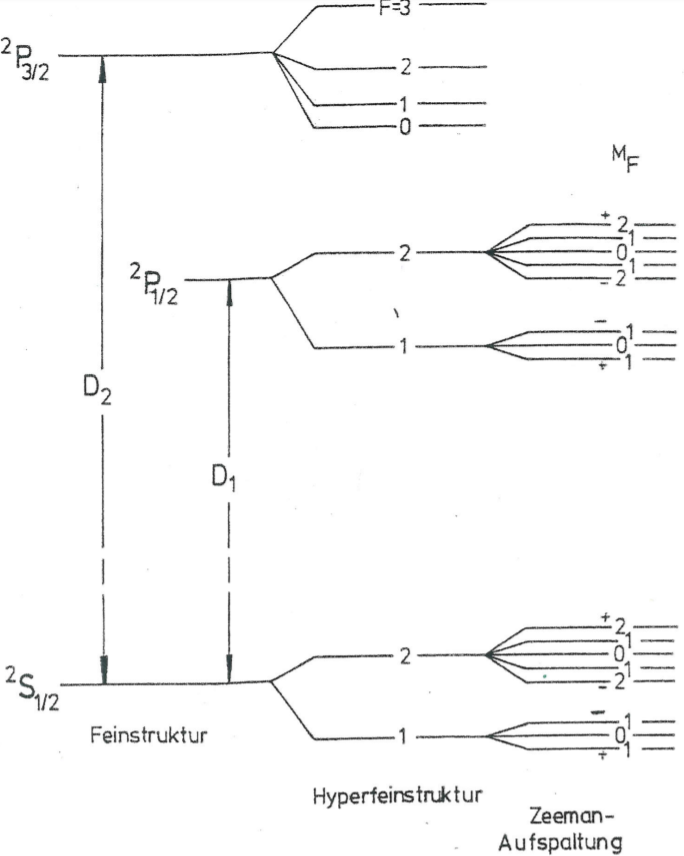
\includegraphics[width=0.6\linewidth]{data/Niveau.png}
	\caption{Darstellung der D$_1$ und D$_2$ Übergänge in Rubidium.}
	\label{fig:Energieniveau}
\end{figure}


\noindent
Das Optische Pumpen soll hierbei durch D$_1$-Licht passieren. Die elektronen weden also aus ihrem Grundzustand $^2$S$_{1/2}$ in den ersten angeregten
Zustand $^2$P$_{1/2}$ gehoben. Dabei ist zu beachten, dass es sich um rechtszirkular polarisierte Photonen handelt. Desshalb folgt der Übergang der
Auswahlregel $\Delta M = 1$. Für linkszirkular polarisierte Photonen würde dementsprechen $\Delta M=-1$ und für Linearpolarisierte $\Delta M=0$ gelten.
Übergänge durch rechtszirkular polarisierte Photenen werden $\sigma^+$-, durch linkszirkular polarisierte Photonen $\sigma^-$- und durch linearpolarisierte
Photonen $\pi$-Übergänge genannt.
\newline
Da es sich bei der D$_1$-Strahlung nun um rechtszirkular polarisiertes Licht handelt, werden alle Grundzustandsniveaus angeregt, die nicht gegen die Auswahlregel $\Delta M=1$
verstoßen würden. Wenn die Photonen dann aus ihrem angeregten Zustand zurück in den Grundzustand übergehen, sind alle Grundzustandsniveaus erlaubt. Es werden sich also nach
Ablauf einiger Zeit die Elektronen in dem Zustand sammeln, aus dem sie nicht wieder angeregt werden können. Das Atom ist dann für die rechtszirkular polarisierten Photonen
transparent und die Besetzungsinversion erreicht. Diese Besetzungsinversion lässt sich dann durch ein hochfrequentes RF-Feld aufheben, falls dieses mit der Resonanzfrequenz
der Zeeman-Niveauübergänge $\nu_\text{res}$ oszilliert. Für $\nu_\text{res}$ gilt

\begin{equation}
    \nu_\text{res}=g_F\mu_0B/\text{h}.
  \end{equation}

\noindent
In diesem Falle würden durch das RF-Feld induzierte Emissionen stattfinden, die die Besetzungsinversion und somit die Transparenz des Rubidiumdampfes aufheben.
Ein Beispielhafter Verlauf für die Transparenz in Abhängigkeit der RF-Feldstärke ist in \autoref{fig:verlauf} dargestellt. $B_\text{m}$ ist hierbei die Resonanzstelle.


\begin{figure}[H]
  \centering
  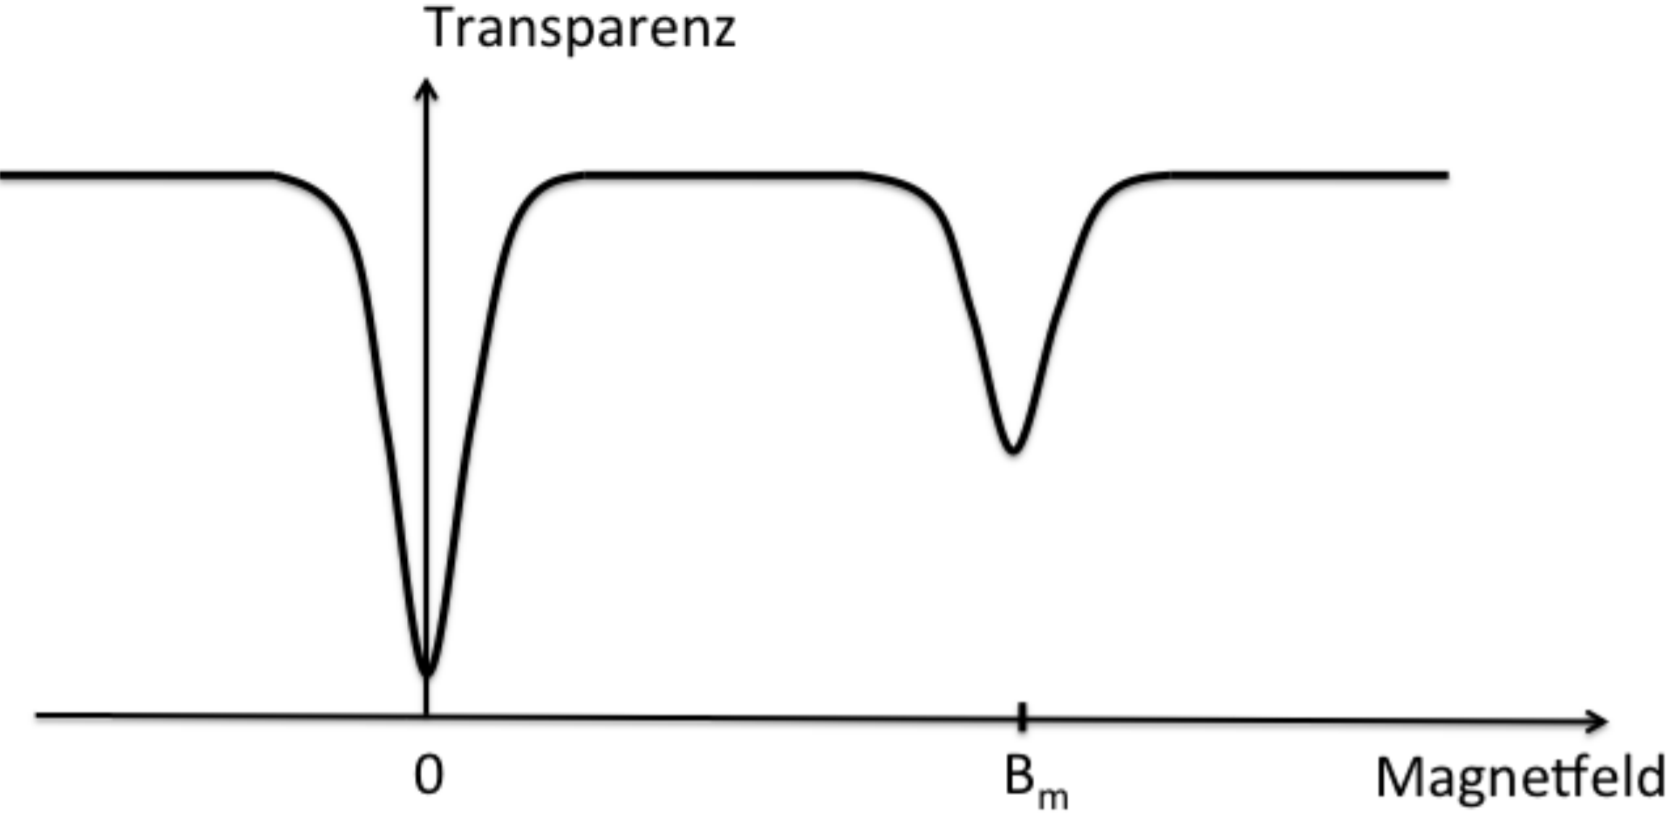
\includegraphics[width=0.5\textwidth]{data/Verlauf.png}
  \caption{Darstellungs der Transparenzänderung einer Rubidiumdampfzelle bei Änderung der Feldstärke eines RF-Feldes.}
  \label{fig:verlauf}
\end{figure}.


\subsection{Der quadratische Zeeman-Effekt}
\label{subsec:QuadZeeman}

Bei der Berechnung des Zeeman-Effekts für starke Magnetfelder müssen quadratische Terme berücksichtigt werden. Die hieraus resultierenden Energiedifferenzen der
Niveaus sind dann gegeben durch:

\begin{equation}
  W = g_F\mu_\text{0}B+g^2_F\mu^2_\text{0}B^2\frac{1-2M_F}{\upDelta E_\text{Hyp}}.
  \label{eq:quadratisch}
\end{equation}

\noindent
hierbei beschreibt $\upDelta E_\text{Hyp}$ die Energiedifferenz der Hyperfeinstrukturniveaus.
